\documentclass{beamer}
\usetheme{Hannover}
\usecolortheme{spruce}
\usepackage{media9}
\usepackage{color}
\title[\color{white}{Project N°2}]{A HIGH-ORDER DISCONTINUOUS GALERKIN METHOD FOR THE BIDOMAIN PROBLEM OF CARDIAC ELECTROPHYSIOLOGY}
\subtitle{Project N°2}
\author[]{\small{\textit{Supervisors: Christian Vergara, Paola Antonietti}}\\ \vspace{5mm} Federica Botta, Matteo Calafà}
\institute[Politecnico di Milano]{Course of Numerical Analysis for Partial Differential Equations}
\date{A.Y. 2020/2021}
\logo{
\includegraphics[height=1cm]{logo_polimi.png}}
\begin{document}

\frame{\titlepage}

\begin{frame}
\frametitle{Table of Contents}
\tableofcontents
\end{frame}

\begin{frame}
\section{Introduction}
\frametitle{The physical problem}
\begin{center}
Mechanical contraction of the human heart\\

$\downarrow$

Electrical activation of the cardiac cells\\

$\downarrow$

Continuos electrical diffusion over the entire cardiac surface.\\
\end{center}
\vspace{1cm}
\begin{columns}
            \begin{column}{0.5\textwidth}
                  \begin{figure}[t]
                  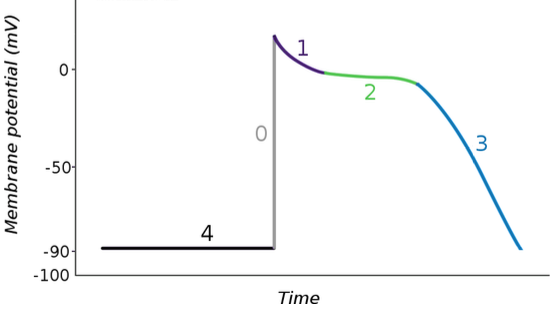
\includegraphics[width = 0.8\textwidth]{./potential_cycle.png}
                  \centering
                  \end{figure}
            \end{column}
            \begin{column}{0.5\textwidth}  
            \begin{figure}[t]
                  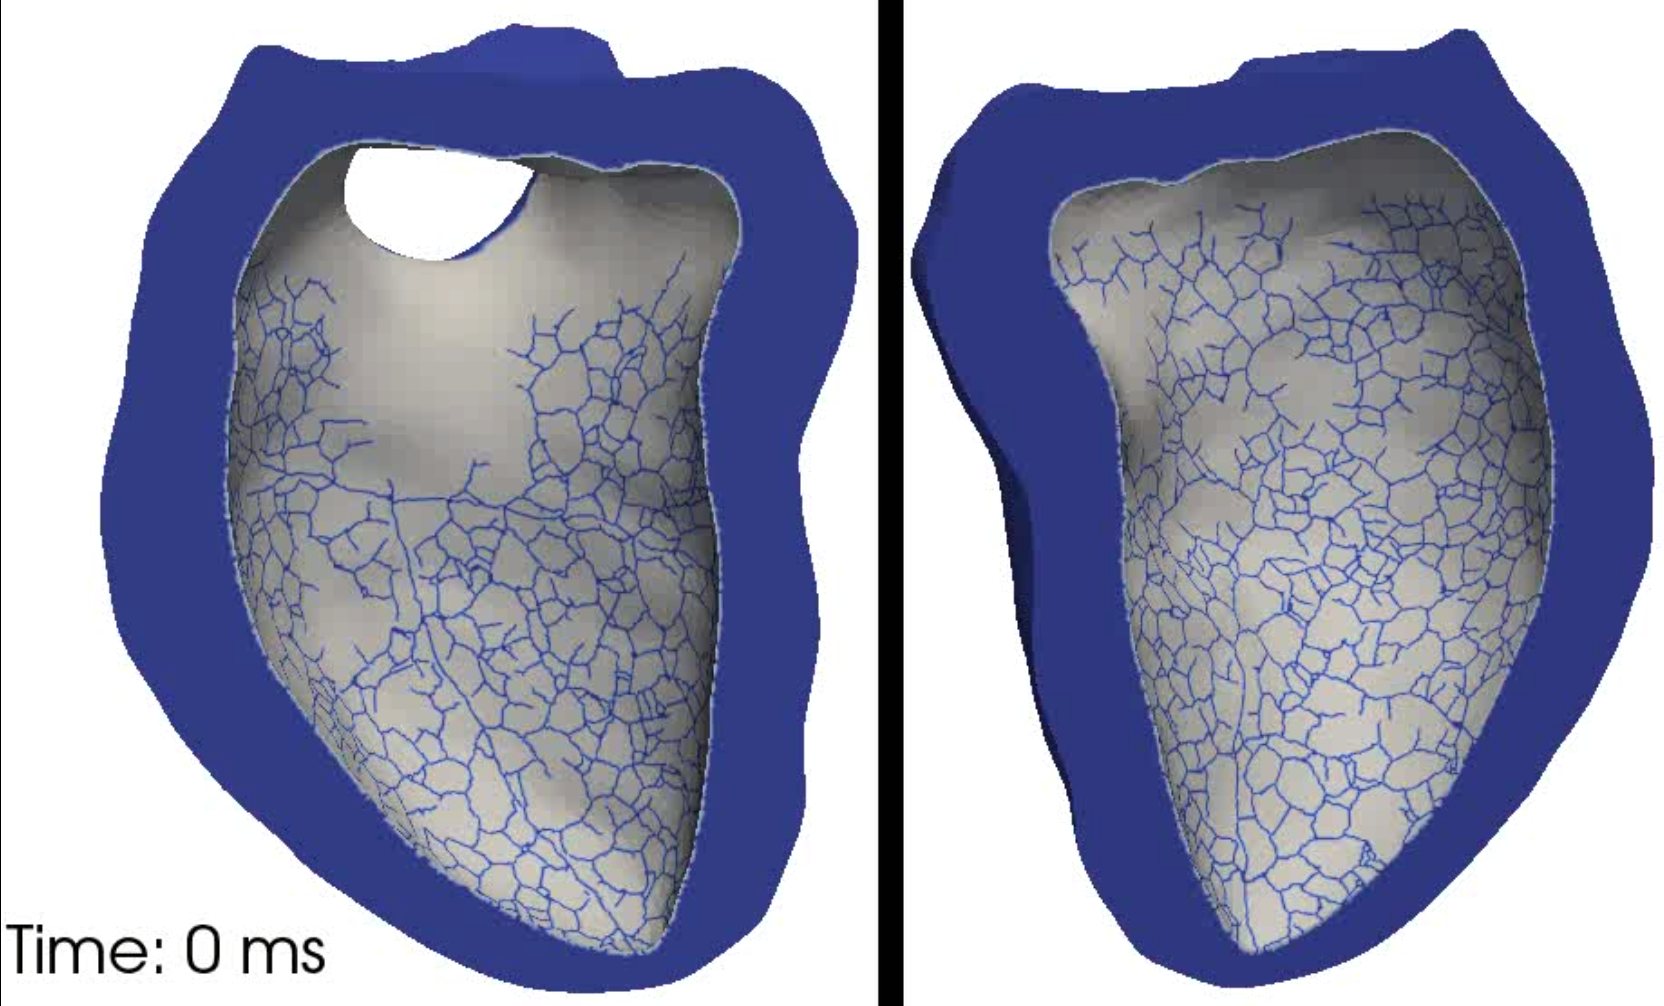
\includegraphics[width = 0.8\textwidth]{./image.png}
                  \centering
                  \end{figure} 
                  %\includemedia[width=5cm,height=3cm,addresource=Video_Presentazione.avi,activate=onclick]{}{VPlayer.swf}
                  \centering
            \end{column}
     \end{columns}
\end{frame}

\end{document}
